\chapter{Communication Systems}

\section{What is Communication?}

\textbf{Communication} (from Latin \emph{communicare}, ``to share'') is the act of conveying information from one entity to another using mutually understood sign and symbols.

\textbf{Information} is the knowledge which is being conveyed from the source to the recipient. Information results in increased knowledge at the recipient's side.

Many research areas concern with communication and information:
\begin{itemize}
	\item Information theory: Quantification, storage, communication and information in general
	\item Communication studies: Human communication
	\item Linguistics: Language as a carrier of information
	\item Biosemiotics: Communication in and between living organisms
	\item ...
\end{itemize}

Communication and information are general terms. \textbf{Digital communication} concerns with the technology of conveying information using discrete signals. A \textbf{digital communication system} is a set of components and processes which implement digital communication. The signals carrying the information in a digital communication system are usually electromagnetic waves.


\section{Objectives and Distinction from Other Subjects}

This course will provide an understanding of how a digital communication system can be described. You will learn methods to describe information in their physical form as signals as well as system components. 

The theory of digital communication system is strongly connected to other subjects, for example:
\begin{itemize}
	\item Information and coding theory
	\item Computer networks
	\item Statistics
	\item Signals and systems
	\item Microwave engineering
	\item Electronics
\end{itemize}
There are courses at this university which give you a deeper insight into these subjects.


\section{Components of A Communication System}


\subsection{Communication Model}

%\todo{citation}
Claude Shannon and Warren Weaver were engineers at the Bell Telephone Labs, USA. They developed the \textbf{Shannon-Weaver Model} (Figure \ref{fig:ch01:shannon_weaver_model}).

\begin{figure}[H]
	\centering
	\begin{tikzpicture}
		\draw node[draw, block](Source){Information\\ source};
		\draw node[draw, block, right=of Source](STrans){Transducer\\ (sender)};
		\draw node[draw, block, right=of STrans](TX){Transmitter};
		\draw node[draw, block, below right=of TX](Ch){Transmission\\ channel};
		\draw node[draw, block, below left=of Ch](RX){Receiver};
		\draw node[draw, block, left=of RX](RTrans){Transducer\\ (recipient)};
		\draw node[draw, block, left=of RTrans](Sink){Information\\ sink};
		
		\draw[-latex] (Source) -- node[midway, align=center, above]{a} (STrans);
		\draw[-latex] (STrans) -- node[midway, align=center, above]{b} (TX);
		\draw[-latex] (TX) -| node[midway, align=center, above left]{c} (Ch);
		\draw[-latex] (Ch) |- node[midway, align=center, above left]{d} (RX);
		\draw[-latex] (RX) -- node[midway, align=center, above]{e} (RTrans);
		\draw[-latex] (RTrans) -- node[midway, align=center, above]{f} (Sink);
	\end{tikzpicture}
	\caption{Shannon-Weaver model of communication}
	\label{fig:ch01:shannon_weaver_model}
\end{figure}

\begin{description}
	\item[Information source] The information is created here.
	\item[Signal a] The original information is represented in physical form by a signal.
	\item[Transducer (sender)] The transducer converts the signal from one physical form to another.
	\item[Signal b] The signal is in a form which can be processed by the transmitter.
	\item[Transmitter] The information is modulated on a carrier, which can be transmitted through the transmission channel.
	\item[Signal c] The information is modulated on a carrier and can pass through the transmission channel.
	\item[Tansmission channel] The physical system through which the modulated information passes. Transmission channels are noisy and add disturbances to the information.
	\item[Signal d] It is basically the Signal c. However, noise and disturbances have been added.
	\item[Receiver] The receiver extracts the information from the carrier. Information must be reconstructed from the noisy input signal.
	\item[Signal e] The output signal of the receiver.
	\item[Transducer (recipient)] The signal must be converted into a physical form which can be processed by the information sink.
	\item[Signal f] The signal carries the information in a form which can be used by the information sink.
	\item[Information sink] The endpoint of the information. It uses the information to gain knowledge.
\end{description}

\paragraph{Example: Cell phone}

\begin{enumerate}
	\item The information source is the brain.
	\item Electrical impulses and molecules are conveyed by the nerves to the vocal cords (transducer 1). Vocal cords convert the signals to sound.
	\item The sound is converted to an electrical signal by a microphone (transducer 2).
	\item The electrical pulses are modulated on a radio carrier (transmitter).
	\item Radio waves are transmitted over the air (transmission channel).
	\item A noisy signal is received. The receivers demodulates the information from the radio carrier.
	\item The analogue electrical signal is converted into sound by a speaker (transducer 3).
	\item The sound reaches the ear that converts them to electrical pulses (transducer 4).
	\item Electrical impulses and molecules are conveyed by the nerves to the brain (information sink).
\end{enumerate}


\subsection{Classification of Signals}

A signal conveys information in a form that can be processed by components of the communication systems.

\begin{figure}[H]
	\centering
	\begin{tikzpicture}
		\draw node[block](Main){\textbf{Signals carrying}\\ \textbf{information}};
		\draw node[block, below left=of Main](Analogue){Analogue};
		\draw node[block, below right=of Main](Digital){Digital};
		\draw node[block, below left=of Analogue](TimeCont){Time\\ continuous};
		\draw node[block, below right=of Analogue](TimeDis){Time\\ discrete};
		
		\draw [-latex] (Main) -- (Analogue);
		\draw [-latex] (Main) -- (Digital);
		\draw [-latex] (Analogue) -- (TimeCont);
		\draw [-latex] (Analogue) -- (TimeDis);
	\end{tikzpicture}
	\caption{Classification of signals carrying information}
	\label{fig:ch01:signals_classif}
\end{figure}

\paragraph{Analogue signals.}

Analogue signals are represented by values out of a continuous range (\emph{value-continuous}). The range can be limited. However, each real value in this range can be taken.

Examples:
\begin{itemize}
	\item Acoustic signals (speech, sound)
	\item Electric signals (voltage, current)
	\item Light signals (microscope, photograph)
\end{itemize}

Analogue signals can be time-continuous or time-discrete. \emph{Time-continuity} means that the signal is defined at any real point of time. A \emph{time-discrete} signal is only defined at certain time instances. The number of time instances can be unlimited. However, the signal is not defined between two time points.

\begin{figure}[H]
	\centering
	\begin{adjustbox}{scale=0.8}
		\begin{tikzpicture}
			\draw node[draw, block](Continuous){Value-continuous,\\ time-continuous\\ signal};
			\draw node[draw, block, right=3cm of Continuous](Sampled){Value-continuous,\\ time-discrete\\ signal};
			\draw node[draw, block, right=3cm of Sampled](Digital){Value-discrete,\\ time-discrete\\ signal};
			
			\draw [-latex] (Continuous) -- node[midway, align=center, above]{Sampling} (Sampled);
			\draw [-latex] (Sampled) -- node[midway, align=center, above]{Quantization} (Digital);
			
			\draw[decorate, decoration={brace, amplitude=3mm, mirror}] ([yshift=-5mm] Continuous.south west) -- ([yshift=-5mm] Sampled.south east) node[midway, below, yshift=-3mm]{\textbf{Analogue}};
			\draw[decorate, decoration={brace, amplitude=3mm, mirror}] ([yshift=-5mm] Digital.south west) -- ([yshift=-5mm] Digital.south east) node[midway, below, yshift=-3mm]{\textbf{Digital}};
		\end{tikzpicture}
	\end{adjustbox}
	\caption{Conversion from analogue to digital signals}
	\label{fig:ch01:signals_sampling}
\end{figure}

\begin{figure}[H]
	\centering
	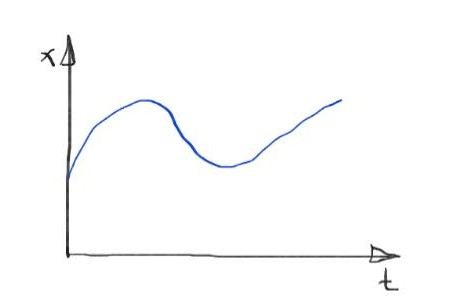
\includegraphics{../chapter01/Signal_Analogue.jpg}
	\caption[An analogue, value-continuous, time-continuous signal]{An analogue, value-continuous, time-continuous signal. Both time and value can be any real number.}
	\label{fig:ch01:Signal_Analogue}
\end{figure}

\begin{figure}[H]
	\centering
	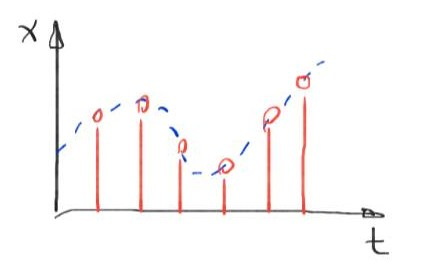
\includegraphics{../chapter01/Signal_TimeDiscr.jpg}
	\caption[An analogue, value-continuous, but time-discrete signal]{An analogue, value-continuous, but time-discrete signal. Only certain time points are valid, but the values can be any real number.}
	\label{fig:ch01:Signal_TimeDiscr}
\end{figure}

\paragraph{Digital signals.}

Digital signals are both time-discrete and value-discrete. \emph{Value-discrete} means that they can take only one state out of a limited set of states.

\begin{figure}[H]
	\centering
	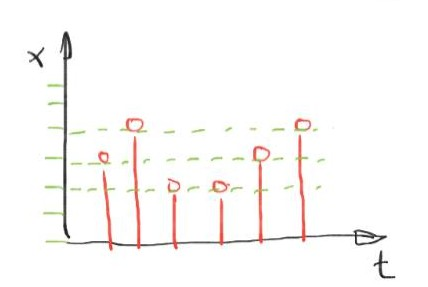
\includegraphics{../chapter01/Signal_Digital.jpg}
	\caption[A digital, value-discrete, time-discrete signal]{A digital, value-discrete, time-discrete signal. Only certain time points and a limited set of values are valid.}
	\label{fig:ch01:Signal_Digital}
\end{figure}

Examples:
\begin{itemize}
	\item Text letters
	\item Morse code
	\item Coded data
\end{itemize}

\textit{Remark:} In fact, the physical form of a digital signal is again an analogue signal. A binary signal can take the discrete states ``high'' and ``low''. If the signal is on a wire, its states are represented by voltage levels, for example \SI{0}{V} and \SI{3.3}{V}. However, if processed by a digital system, the physical representation is of minor importance. Only the discrete, logical states are considered.

A special kind of digital signal is the \textbf{binary signal}. It has two discrete states.


\subsection{Transmission Channels}

Digital communication systems employ electromagnetic waves to convey information. Therefore, only transmission channels transporting electromagnetic waves are considered.

\begin{figure}[H]
	\centering
	\begin{tikzpicture}
	\draw node[block](Main){\textbf{Transmission}\\ \textbf{channels}};
	\draw node[block, below left=of Main](Wired){Wired\\ channels};
	\draw node[block, below right=of Main](Wireless){Wireless\\ channels};
	
	\draw [-latex] (Main) -- (Wired);
	\draw [-latex] (Main) -- (Wireless);
	\end{tikzpicture}
	\caption{Classification of transmission channels}
	\label{fig:ch01:trans_ch_classif}
\end{figure}

\paragraph{Wired Channels.}

The electromagnetic wave propagates along a transmission line.

Examples of transmission lines:
\begin{itemize}
	\item Cables
	\begin{itemize}
		\item Two wire, twisted pair
		\item Coaxial cable
	\end{itemize}
	\item Waveguides
	\item Planar lines (on printed circuit boards or integrated circuits)
	\begin{itemize}
		\item Microstrip
		\item Coplanar waveguide
	\end{itemize}
	\item Glass fibre (light is an electromagnetic wave, too)
\end{itemize}

\paragraph{Wireless Channels.}

The electromagnetic wave is not bound to a transmission line. It propagates through the space. A medium is not necessary. Electromagnetic wave can also travel through vacuum.


\section{Computer Networks}


This course focuses on the technologies which convey information between endpoints, using electromagnetic waves. The information, being conveyed, are called \textbf{data}. The handling of the data is a subject of computer science, especially \emph{computer networks}. Since data processing is a part of digital communication systems, too, this digression shall give an overview about the employed concepts.


\subsection{Protocols}

Modern communication systems convey information world-wide. These communication links are established over myriads of devices, which form a network. The biggest computer network is the internet.

These devices mainly operate automatically without human interaction. Therefore, they are required to follow certain rules, which are called \textbf{communication protocols}. Protocols define
\begin{itemize}
	\item the structure and semantics of data,
	\item synchronization of communication, and
	\item possible error recovery methods.
\end{itemize}

Protocols are standardized and must be implemented in every device, which interacts with other devices. Important standardization organizations are:
\begin{itemize}
	\item The non-profit organization \textbf{Internet Engineering Task Force} (IETF) issues standards concerning the internet. The standards are called \emph{Request For Comment} (RFC) and are available for everyone for free. Example standards: Internet Protocol (IP), Hypertext Transfer Protocol (HTTP)
	\item The \textbf{Institute of Electrical and Electronics Engineers} (IEEE) has standards committees which develop and publish standards. With respect to the internet, the IEEE\,802 LAN/MAN Standards Committee is the most important one. Example standards: IEEE\,802.11 (Wifi)
	\item The \textbf{European Telecommunications Standards Institute} (ETSI) is an independent, non-profit standardization organization. It is recognized by the European Council and officially responsible for standardization of information and communication technologies in Europe. Example standards: 3G (cell phone system), 4G (cell phone system), TETRA (professional mobile radio system)
\end{itemize}


\subsection{OSI Model}

There are many task which a digital communication systems must accomplish.
\begin{itemize}
	\item An application processes user input and displays data to the user.
	\item The application data must be reliably transferred over a network with many nodes.
	\item The network is shared with other users and applications.
	\item The network consists of many links using different physical transmission channels, for example, wired and wireless.
\end{itemize}
For each task, there are communication protocols to solve it. Communication protocols are grouped by the task which they fulfil. There is an increasing level of abstraction from the physical link to the application data. The \textbf{OSI Model} (Figure \ref{fig:ch01:osi_model}) defines a layer structure for classifying communication protocols, which regards the level of abstraction.

\begin{figure}[H]
	\centering
	\begin{tikzpicture}[
		layer/.style={
			rectangle,
			minimum height=1cm,
			minimum width=8cm
		}
	]
		\draw node[draw, layer](L7){Application layer};
		\draw node[draw, layer, below=0 of L7](L6){Presentation layer};
		\draw node[draw, layer, below=0 of L6](L5){Session layer};
		\draw node[draw, layer, below=0 of L5](L4){Transport layer};
		\draw node[draw, layer, below=0 of L4](L3){Network layer};
		\draw node[draw, layer, below=0 of L3](L2){Data link layer};
		\draw node[draw, layer, below=0 of L2](L1){Physical layer};
		
		\node [anchor=east, align=right] at([xshift=-5mm] L7.west) {Layer 7};
		\node [anchor=east, align=right] at([xshift=-5mm] L6.west) {Layer 6};
		\node [anchor=east, align=right] at([xshift=-5mm] L5.west) {Layer 5};
		\node [anchor=east, align=right] at([xshift=-5mm] L4.west) {Layer 4};
		\node [anchor=east, align=right] at([xshift=-5mm] L3.west) {Layer 3};
		\node [anchor=east, align=right] at([xshift=-5mm] L2.west) {Layer 2};
		\node [anchor=east, align=right] at([xshift=-5mm] L1.west) {Layer 1};
		
		\filldraw[fill=gray!60, draw=none] ([xshift=10mm, yshift=3mm] L7.north east) -- node[midway, above, anchor=south, align=center]{Level of\\ abstraction} ([xshift=15mm, yshift=3mm] L7.north east) -- ([xshift=12.5mm, yshift=-3mm] L1.south east);
	\end{tikzpicture}
	\caption{OSI Model with seven layers}
	\label{fig:ch01:osi_model}
\end{figure}

\begin{table}[H]
	\caption{Description of the layers of the OSI Model (Figure \ref{fig:ch01:osi_model}). The protocol data unit is the information }
	\begin{tabular}{|l|l|p{0.5\linewidth}|}
		\hline
		Layer & PDU & Function \\
		\hline
		\hline
		7: Application & Data & Processing user inputs, displaying data, providing services \\
		\hline
		6: Presentation & Data & Translation between network service and application (encryption, compression, etc.) \\
		\hline
		5: Session & Data & Managing sessions (retaining the communication state across multiple contacts) \\
		\hline
		4: Transport & Datagram, Segment & Reliable communication (segmentation, multiplexing, data loss detection) \\
		\hline
		3: Network & Packet & Data transfer across multiple nodes (addressing, routing, traffic control) \\
		\hline
		2: Data link & Frame & Transmission between two devices (medium access, flow control) \\
		\hline
		1: Physical & Symbol & Transmission over a physical medium \\
		\hline
	\end{tabular}
\end{table}

Each protocol has a standardized interface exposed to the upper layer, called \textbf{Service Access Point}. They allow an upper layer protocol to execute functions of the lower layer protocol. These functions are, for example:
\begin{itemize}
	\item Sending or receiving data
	\item Control operations
	\item Network registration and de-registration
\end{itemize}

Protocol layers add own information to the data received from the upper layer. This additional information is required to provide the protocol's functionality. For example, the Internet Protocol (IP) needs to add the source and destination address, so that the packet can be routed to the correct endpoint. One can imagine this like data which is written on a letter, which is put into an envelope, which itself is put into another envelope, and so on.

\begin{figure}[H]
	\centering
	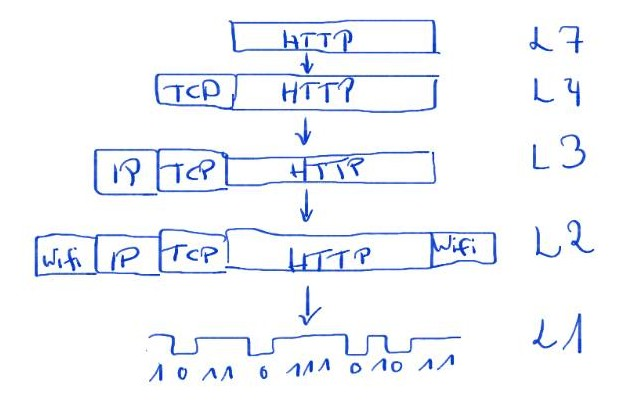
\includegraphics{../chapter01/Frame_Wrapping.jpg}
	\caption{Principle of adding more information in each protocol layer}
	\label{fig:ch01:frame_construction}
\end{figure}

Communication protocols may be exchanged in one layer without affecting the functionality of the other layers. For example, HTTP operates on TCP/IP. But the Internet Protocol (IP) works on multiple physical links like Ethernet (IEEE\,802.3), Wifi (IEEE\,802.11) or 4G. The transmission media can even change along the communication path. Information travlling through the internet experience lots of \textbf{media changes}.


\begin{figure}[H]
	\centering
	\caption{Media change on the internet. }
	\label{fig:ch01:media_changes}
\end{figure}

This course on digital communication systems mainly considers the physical layer (layer 1) and the data link layer (layer 2). This physical layer converts the information to physical signals which then leave the device to be transmitted over a physical transmission channel. Networks, which are enabled by protocols of layer 3 and above, are outside the scope of this course.


\subsection{Network Topologies}

\begin{itemize}
	\item \textbf{Ring}
	\item \textbf{Star}
	\item \textbf{Tree}
	\item \textbf{Chain}
	\item \textbf{Bus}
	\item \textbf{Mesh}, special form \emph{Full Mesh}
\end{itemize}

